\documentclass{article}
\usepackage[utf8]{inputenc}
\usepackage{mathtools, amsthm, amsmath, amssymb, graphicx, verbatim}
%\usepackage[thmmarks, thref, amsthm]{ntheorem}
\usepackage{color}
\usepackage{wrapfig}
\usepackage{subcaption}
\usepackage[colorinlistoftodos,textsize=tiny]{todonotes} % need xargs for below
%\usepackage{accents}
\usepackage{bbm}
\usepackage{xspace}

\usetikzlibrary{calc}
\newcommand{\Comments}{1}
\newcommand{\mynote}[2]{\ifnum\Comments=1\textcolor{#1}{#2}\fi}
\newcommand{\mytodo}[2]{\ifnum\Comments=1%
  \todo[linecolor=#1!80!black,backgroundcolor=#1,bordercolor=#1!80!black]{#2}\fi}
\newcommand{\raf}[1]{\mynote{green}{[RF: #1]}}
\newcommand{\raft}[1]{\mytodo{green!20!white}{RF: #1}}
\newcommand{\jessie}[1]{\mynote{purple}{[JF: #1]}}
\newcommand{\jessiet}[1]{\mytodo{purple!20!white}{JF: #1}}
\newcommand{\bo}[1]{\mynote{blue}{[Bo: #1]}}
\newcommand{\botodo}[1]{\mytodo{blue!20!white}{[Bo: #1]}}
\ifnum\Comments=1               % fix margins for todonotes
  \setlength{\marginparwidth}{1in}
\fi


\newcommand{\reals}{\mathbb{R}}
\newcommand{\posreals}{\reals_{>0}}%{\reals_{++}}
\newcommand{\dom}{\mathrm{dom}}

\newcommand{\prop}[1]{\Gamma[#1]}
\newcommand{\eliccts}{\mathrm{elic}_\mathrm{cts}}
\newcommand{\eliccvx}{\mathrm{elic}_\mathrm{cvx}}
\newcommand{\elicpoly}{\mathrm{elic}_\mathrm{pcvx}}
\newcommand{\elicembed}{\mathrm{elic}_\mathrm{embed}}

\newcommand{\cell}{\mathrm{cell}}

\newcommand{\abstain}[1]{\mathrm{abstain}_{#1}}
\newcommand{\mode}{\mathrm{mode}}

\newcommand{\simplex}{\Delta_\Y}

% alphabetical order, by convention
\newcommand{\C}{\mathcal{C}}
\newcommand{\D}{\mathcal{D}}
\newcommand{\E}{\mathbb{E}}
\newcommand{\F}{\mathcal{F}}
\newcommand{\I}{\mathcal{I}}
\newcommand{\R}{\mathcal{R}}
\newcommand{\X}{\mathcal{X}}
\newcommand{\Y}{\mathcal{Y}}

\newcommand{\inprod}[2]{\langle #1, #2 \rangle}%\mathrm{int}(#1)}
\newcommand{\inter}[1]{\mathring{#1}}%\mathrm{int}(#1)}
%\newcommand{\expectedv}[3]{\overline{#1}(#2,#3)}
\newcommand{\expectedv}[3]{\E_{Y\sim{#3}} {#1}(#2,Y)}
\newcommand{\toto}{\rightrightarrows}
\newcommand{\strip}{\mathrm{strip}}
\newcommand{\trim}{\mathrm{trim}}
\newcommand{\fplc}{finite-piecewise-linear and convex\xspace} %xspace for use in text
\newcommand{\conv}{\mathrm{conv}}
\newcommand{\ones}{\mathbbm{1}}
\DeclarePairedDelimiter\ceil{\lceil}{\rceil}

\newcommand{\Ind}{\mathbf{1}}

\DeclareMathOperator*{\argmax}{arg\,max}
\DeclareMathOperator*{\argmin}{arg\,min}
\DeclareMathOperator*{\arginf}{arg\,inf}
\DeclareMathOperator*{\sgn}{sgn}


\newtheorem{theorem}{Theorem}
\newtheorem{lemma}{Lemma}
\newtheorem{claim}{Claim}
\newtheorem{corollary}{Corollary}

\theoremstyle{definition}
\newtheorem{definition}{Definition}

\begin{document}

\bo{Not sure how to integrate this notation into the rest of the document.}

Let some norm $\|\cdot\|$ on finite-dimensional Euclidean space be given.
Given a set $T$ and a point $u$, let $d(T,u) = \inf_{t \in T} \|t-u\|$.

Given two sets $T,T'$, let $d(T,T') = \inf_{t\in T, t' \in T'} \|t-t'\|$.

Let the ``thickening'' $B(T,\epsilon)$ be defined as
  \[ B(T,\epsilon) = \{u \in \R' : d(T,u) < \epsilon \} . \]

We are given an original loss $\ell$ with property $\gamma$ and finite report space $\R$; and a polyhedral embedding with loss $L$, property, $\Gamma$, report space $\R' \subseteq \reals^d$, and embedding points $\{u_r : r \in \R\}$.


Let $\mathcal{S} \subseteq 2^{\R}$ be defined as $\mathcal{S} = \{\gamma(p) : p \in \Delta_{\Y}\}$.
In other words, for each $p$, we take the set of optimal reports $R = \gamma(p) \subseteq \R$, and we add $R$ to $\mathcal{S}$.

Let $\mathcal{U} \subseteq 2^{\reals^d}$ be defined as $\mathcal{U} = \{\Gamma(p) : p \in \Delta_{\Y}\}$.

\begin{lemma} \label{lemma:U-convex-closed}
  $\mathcal{U}$ is a finite set, and each element $U$ is a closed, convex polyhedron.
\end{lemma}
\begin{proof}
  \raf{I updated the main doc to include a proof of exactly this statement.  It made me realize that the existing proof was wrong, and this is actually the right thing to show anyway!}
  \bo{More of a sketch right now}
  Let $p$ be in the interior of the simplex.
  For any such $p$, the polyhedral expected loss $L(\cdot;p)$ projects down to the same fixed power diagram over $\reals^d$.
  The minimizer of a polyhedral loss is always the projection of some face of the polyhedron, \bo{cite} so there are a finite number of possible minimizers and each is a closed, convex polyhedron (being a member of the power diagram or an intersection of members).
  Now for $p$ not in the interior, consider each of finitely many subsets of the outcome space and restrict $p$ to have support on this subset; repeat the above arguments.
  The total number of report sets $U$ is still finite, each a closed, convex polyhedron.
\end{proof}

\begin{lemma} \label{lemma:U-surject}
  There is a surjection from $\mathcal{U}$ to $\mathcal{S}$ where $U \mapsto R$ if, for some $p$, we have $\gamma(p) = U$ and $\Gamma(p) = R$.
  We write $R_U$ for the value of this map at $U$.
\end{lemma}
\begin{proof}
  For each report $r$, write $u_r$ for its embedding point and for each $U \in \mathcal{U}$, let $R_U = \{r : u_r \in U\}$.
  Recall that $\mathcal{U}$ is the collection of sets $U = \gamma(p)$ for some $p$, while $\mathcal{S}$ is the collection of sets $R = \Gamma(p)$ for some $p$.
  By definition of embedding, we have for any $p$ that $u_r \in \Gamma(p) \iff r \in \gamma(p)$.
  So if $U = \Gamma(p)$, we must have $R_U = \gamma(p)$.
  This shows that $R_U \in \mathcal{S}$ for all $U$, and furthermore, the map is surjective because every $R \in \mathcal{S}$ is equal to $R_U$ for some $U \in \mathcal{U}$.
\end{proof}

The next lemma shows that if a subset of $\mathcal{U}$ intersect, then their corresponding report sets intersect as well.
\begin{lemma} \label{lemma:calibrated-pos}
  Let $\mathcal{U}' \subseteq \mathcal{U}$.
  If $\cap_{U\in\mathcal{U}'} U \neq \emptyset$ then $\cap_{U\in\mathcal{U}'} R_U \neq \emptyset$.
\end{lemma}
\begin{proof}
  Let $u \in \cap_{U\in\mathcal{U}'} U$.
  Then there is some $r$ such that $\Gamma_u \subseteq \gamma_r$. \bo{This follows because $L$ embedding $\ell$ implies $L$ indirectly elicits $\ell$. Uses trim.}
  Therefore, if we have $p$ such that $u$, then $r$ is optimal.
  Since $u \in U$, we have $r \in R_U$.
  This holds for all $U \in \mathcal{U}'$, so $r \in \cap_{U\in\mathcal{U}'} R_U$, so it is nonempty.
\end{proof}

%% Bo: I thought this might be useful, but guess not.
%\begin{lemma}
%  Let $\{U_j : j \in \mathcal{J}\}$ be a finite collection of closed, convex sets.
%  If $u \not\in \cap_j U_j$, then for all small enough $\epsilon > 0$, $u \not\in \cap_j B(U_j,\epsilon)$.
%\end{lemma}
%\begin{proof}
%  Consider the collection $\{U_j : j \in \mathcal{J}\}$ and suppose $u \not \in \cap_j U_j$.
%  In particular, there exists some $U$ in the collection such that $u \not\in U$.
%  Because $U$ is closed and convex, that there exists $\epsilon' > 0$ such that $d(U,u) \geq \epsilon'$.
%  So for all $\epsilon < \epsilon'$, we have $u \not\in B(U,\epsilon)$.
%  This implies $u \not\in \cap_j B(U_j,\epsilon)$.
%\end{proof}
%

\begin{lemma} \label{lemma:enclose-halfspaces}
  Let $D$ be a closed, convex polyhedron in $\reals^d$.
  For any $\epsilon > 0$, there exists an open, convex polyhedron $D'$, the intersection of a finite number of open halfspaces, such that
    \[ D \subseteq D' \subseteq B(D,\epsilon) . \]
\end{lemma}
\begin{proof}
  Let $S$ be the standard open $\epsilon$-ball $B(\{\vec{0}\},\epsilon)$.
  Note that $B(D,\epsilon) = D + S$ where $+$ is the Minkowski sum.
%  Now let $S' = \{u : \|u\|_1 < \delta\}$ be the open $\delta$ ball in $L_1$ norm.
%  By equivalence of norms in Euclidean space, \bo{cite} we can take $\delta$ small enough yet positive such that $S' \subseteq S$.
%  By Lemma \ref{lemma:open-plus-closed-poly}, the Minkowski sum $D' = D + S'$ is an open polyhedron, i.e. the intersection of a finite number of open halfspaces.
  Now let $S' = \{u : \|u\|_1 \leq \delta\}$ be the closed $\delta$ ball in $L_1$ norm.
  By equivalence of norms in Euclidean space, \bo{cite} we can take $\delta$ small enough yet positive such that $S' \subseteq S$.
  By standard results, the Minkowski sum of two closed, convex polyhedra, $D'' = D + S'$ is a closed polyhedron, i.e. the intersection of a finite number of closed halfspaces. (A proof: we can form the higher-dimensional polyhedron $\{(x,y,z) : x \in D, y \in S', z = x+y\}$, then project onto the $z$ coordinates.)

  Now, if $T' \subseteq T$, then the Minkowksi sum satisfies $D + T' \subseteq D + T$.
  In particular, because $\emptyset \subseteq S' \subseteq S$, we have
    \[ D \subseteq D'' \subseteq B(D,\epsilon) . \]
  Now let $D'$ be the interior of $D''$, i.e. if $D'' = \{x : Ax \leq b\}$, then we let $D' = \{x: Ax < b\}$.
  We retain $D' \subseteq B(D,\epsilon)$.
  Further, we retain $D \subseteq D'$, because $D$ is contained in the interior of $D'' = D + S'$.
  (Proof: if $x \in D$, then for some $\gamma$, $x + B(\{\vec{0}\},\gamma) = B(x,\gamma)$ is contained in $D + S'$.)
  This proves the lemma.
\end{proof}

\begin{lemma} \label{lemma:thick-nonempty}
  Let $\{U_j : j \in \mathcal{J}\}$ be a finite collection of closed, convex sets with $\cap_{j\in\mathcal{J}} U_j \neq \emptyset$.
  Then there exists  $\epsilon > 0$ such that $\cap_j B(U_j,\epsilon) \subseteq B(\cap_j U_j, \delta)$.
  \raft{FYI, formalized some of the English in both the statement and proof}
\end{lemma}
\begin{proof}
  We induct on $|\mathcal{J}|$.
  If $|\mathcal{J}|=1$, set $\epsilon = \delta$.
  If $|\mathcal{J}|>1$, let $j\in\mathcal{J}$ be arbitrary, let $U' = \cap_{j'\neq j} U_{j'}$, and let $C(\epsilon) = \cap_{j' \neq j} B(U_{j'},\epsilon)$.
  Let $D = U_j \cap U'$.
  We must show that $B(U_j,\epsilon) \cap C(\epsilon) \subseteq B(D,\delta)$.
  By Lemma \ref{lemma:enclose-halfspaces}, we can enclose $D$ strictly within a polyhedron $D'$, the intersection of a finite number of open halfspaces, which is itself strictly enclosed in $B(D,\delta)$.
  (For example, if $D$ is a point, then enclose it in a hypercube, which is enclosed in the ball $B(D,\delta)$.)
%  \raf{We can use the fact that the $U_j$ are all polyhedral here, so $D$ is polyhedral as well.  Now let $B_1()$ be a ball with respect to $\|\cdot\|_1$, and observe that $B_1(D,\delta')$ is therefore also polyhedral for all $\delta'$.  Using norm bounds, we can find a small enough $\delta'$ so that $B_1(D,\delta') \subseteq B(D,\delta)$.}
  We will prove that, for small enough $\epsilon$, $B(U_j,\epsilon) \cap C(\epsilon)$ is contained in $D'$.
  This implies that it is contained in $B(D,\delta)$.

  For each halfspace defining $D'$, consider its complement $F$, a closed halfspace.
  We prove that $F \cap B(U_j,\epsilon) \cap C(\epsilon) = \emptyset$.
  Consider the intersections of $F$ with $U$ and $U'$, call them $G$ and $G'$.
  These are closed, convex sets that do not intersect (because $D$ in contained in the complement of $F$).
  So $G$ and $G'$ are separated by a nonzero distance, so $B(G,\gamma) \cap B(G',\gamma) = \emptyset$ for small enough $\gamma$.
  And $B(G,\gamma) = F \cap B(U_j,\gamma)$ while $B(G',\gamma) = F \cap B(U',\gamma)$.
  This proves that $F \cap B(U_j,\gamma) \cap B(U',\gamma) = \emptyset$.
  By inductive assumption, $C(\epsilon) \subseteq B(U',\gamma)$ for small enough $\epsilon = \epsilon_F$.
  So $F \cap B(U_j,\gamma) \cap C(\epsilon) = \emptyset$.
  We now let $\epsilon$ be the minimum over these finitely many $\epsilon_F$ (one per halfspace).
\end{proof}

\begin{figure}
\caption{Illustration of a special case of the proof of Lemma \ref{lemma:thick-nonempty} where there are two sets $U_1,U_2$ and their intersection $D$ is a point. We build the polyhedron $D'$ inside $B(D,\delta)$. By considering each halfspace that defines $D'$, we then show that for small enough $\epsilon$, $B(U_1,\epsilon)$ and $B(U_2,\epsilon)$ do not intersect outside $D'$. So the intersection is contained in $D'$, so it is contained in $B(D,\delta)$.}
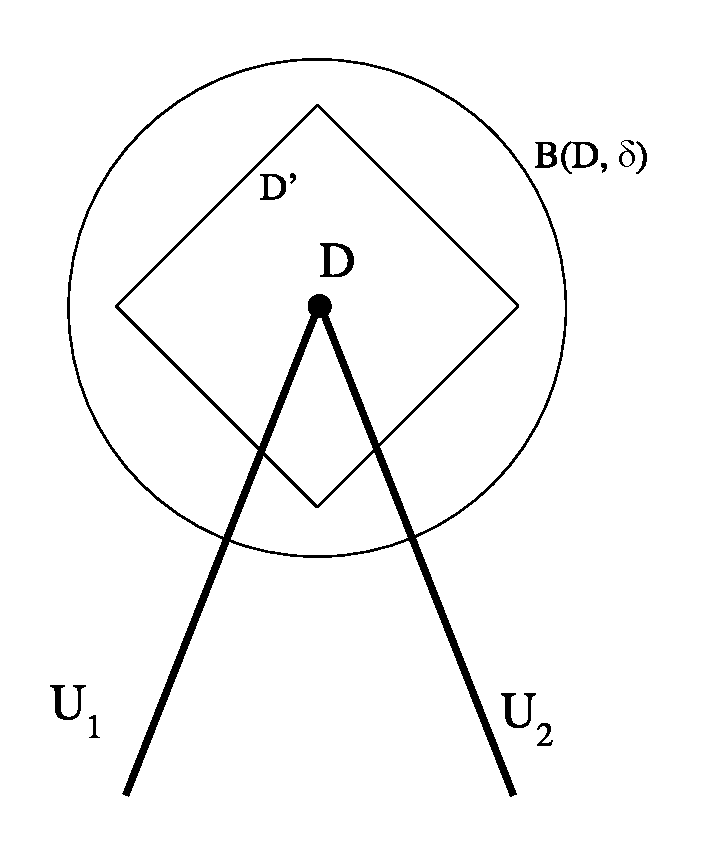
\includegraphics[width=0.24\textwidth]{figs/separated-proof-2} \hfill
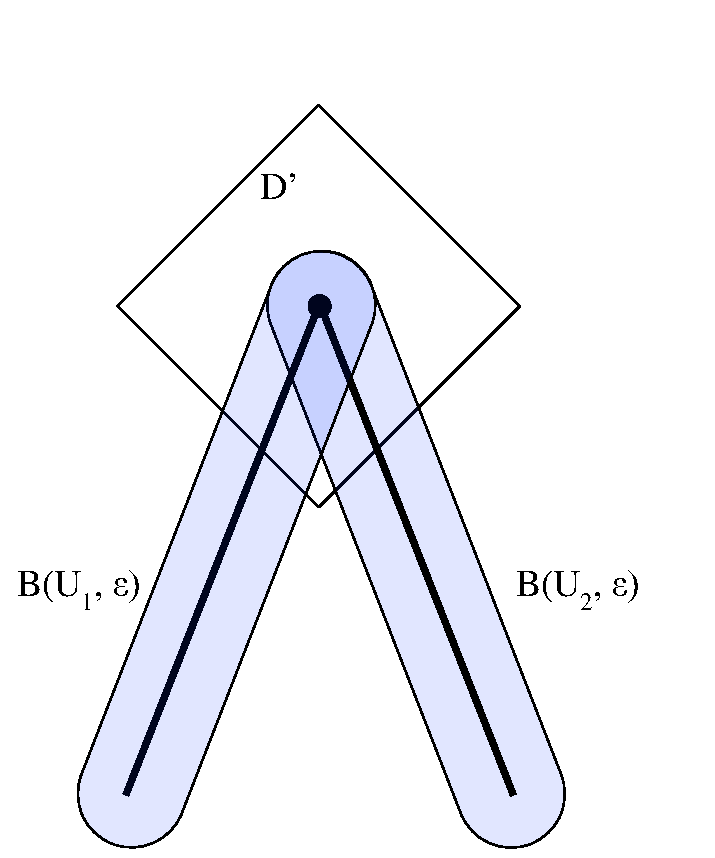
\includegraphics[width=0.24\textwidth]{figs/separated-proof-3} \hfill
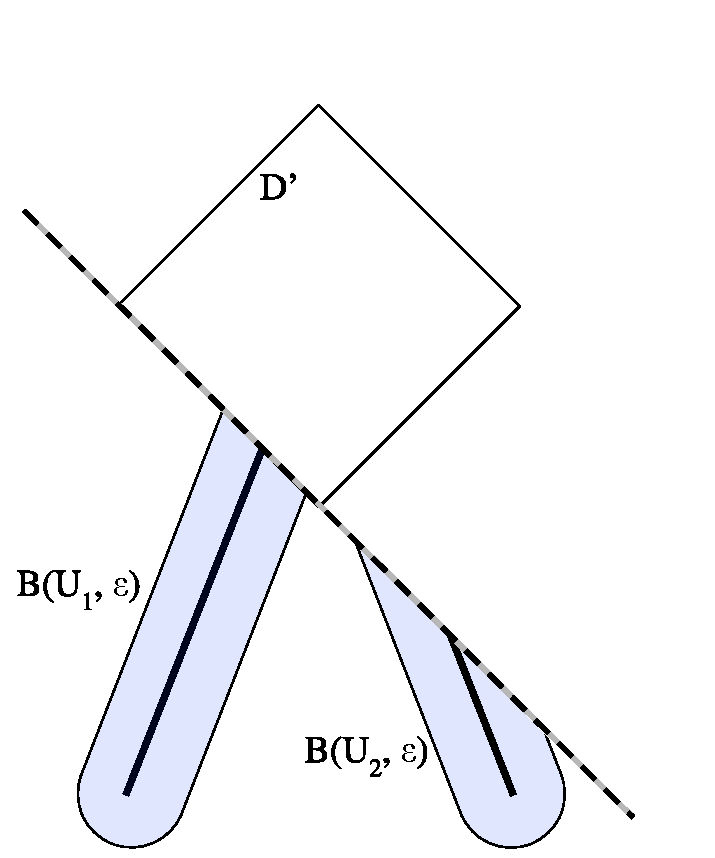
\includegraphics[width=0.24\textwidth]{figs/separated-proof-4} \hfill
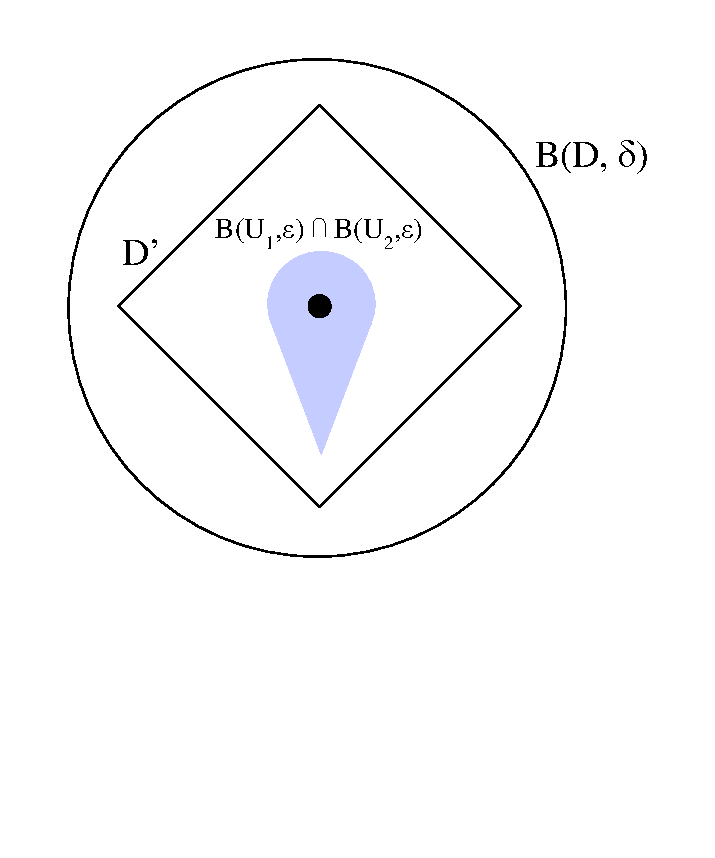
\includegraphics[width=0.24\textwidth]{figs/separated-proof-5}
\end{figure}

\begin{lemma} \label{lemma:thick-empty}
  Let $\{U_j : j \in \mathcal{J}\}$ be a finite collection of nonempty closed, convex sets with $\cap_{j\in\mathcal{J}} U_j = \emptyset$.
  Then for all $\delta > 0$, there exists  $\epsilon > 0$ such that $\cap_{j\in\mathcal{J}} B(U_j,\epsilon) = \emptyset$.
\end{lemma}
\begin{proof}
  By induction on the size of the family.
  Note that the family must have size at least two.
  Let $U_j$ be any set in the family and let $U' = \cap_{j' \neq j} U_{j'}$.
  There are two possibilities.

  The first possibility, which includes the base case where the size of the family is two, is the case $U'$ is nonempty.
  Because $U_j$ and $U'$ are non-intersecting closed convex sets, they are separated by some distance $\epsilon$.
  By Lemma \ref{lemma:thick-nonempty}, for any $\epsilon > 0$, there exists $\delta > 0$ such that $\cap_{j'\neq j} B(U_{j'},\delta) \subseteq B(U', \epsilon/3)$.
  Then we have $B(U_j, \epsilon/3) \cap B(U', \epsilon/3) = \emptyset$.

  The second possibility is that $U'$ is empty.
  This implies we are not in the base case, as the family must have three or more sets.
  By inductive assumption, for small enough $\delta$ we have $\cap_{j' \neq j} B(U_{j'},\delta) = \emptyset$, which proves this case.
\end{proof}

%\begin{lemma} \label{lemma:thick-int}
%  Let $\{U_j : j \in \mathcal{J}\}$ be a finite collection of closed, convex sets.
%  For any $\delta > 0$, there exists an $\epsilon > 0$ such that
%  \[ \cap_j B(U_j,\epsilon) \subseteq B\left(\cap_j U_j, \delta\right)  \]
%  where if $\cap_j U_j = \emptyset$, we interpret the right-hand side as $\emptyset$.
%\end{lemma}
%\begin{proof}
%  \raf{Maybe cleaner to break into to two parts right off the bat: $\cap U_j$ is empty or not?}
%  By induction on the size of the collection.
%  If the size is $1$, set $\epsilon = \delta$.
%  If the size is larger than $1$, let $U_j$ be any member of the collection, let $U' = \cap_{j'\neq j} U_{j'}$, and let $C(\epsilon) = \cap_{j' \neq j} B(U_{j'},\epsilon)$.
%  There are two cases.
%  If $U_j \cap U' = \emptyset$, then we must show that $B(U_j,\epsilon) \cap C(\epsilon) = \emptyset$.
%  Because $U_j,U'$ are both closed and convex, they are separated by some nonzero distance. So for some $\gamma > 0$, we have $B(U_j,\gamma) \cap B(U',\gamma) = \emptyset$.
%  By inductive assumption, for all small enough $\epsilon$, $C(\epsilon) \subseteq B(U',\gamma)$, so we have $B(U_j,\gamma) \cap C(\epsilon) = \emptyset$.
%  Choosing a small enough $\epsilon$ that is also less than $\gamma$ completes this case.
%
%  The other case is that $U_j \cap U' = D$, some nonempty closed convex set.
%  Here we must show that $B(U_j,\epsilon) \cap C(\epsilon) \subseteq B(D, \delta)$.
%  Enclose $D$ in the intersection of a finite number of open halfspaces, which is enclosed in $B(D,\delta)$. \bo{I am claiming this is possible, but I didn't prove it yet...}
%  We will prove that, for small enough $\epsilon$, $B(U_j,\epsilon) \cap C(\epsilon)$ is contained in this same intersection.
%  This implies that it is contained in $B(D,\delta)$.
%
%  For each halfspace, consider its complement $F$, a closed halfspace.
%  We prove that $F \cap B(U_j,\epsilon) \cap C(\epsilon) = \emptyset$.
%  Consider the intersections of $F$ with $U$ and $U'$, call them $G$ and $G'$.
%  These are closed, convex sets that do not intersect (because $D$ in contained in the complement of $F$).
%  So $G$ and $G'$ are separated by a nonzero distance, so $B(G,\gamma) \cap B(G',\gamma) = \emptyset$ for small enough $\gamma$.
%  And $B(G,\gamma) = F \cap B(U_j,\gamma)$ while $B(G',\gamma) = F \cap B(U',\gamma)$.
%  By inductive assumption, $C(\epsilon) \subseteq B(U',\gamma)$ for small enough $\epsilon$.
%  So $F \cap B(U_j,\epsilon) \cap C(\epsilon) = \left(F \cap B(U_j,\epsilon)\right) \cap \left(F \cap C(\epsilon)\right) = \emptyset$ for a small enough $\epsilon$.
%
%  We now take the minimum over these finitely many $\epsilon$'s (one per halfspace).
%\end{proof}
  

\begin{corollary} \label{cor:thick-intersect}
  There exists a small enough $\epsilon > 0$ such that, for any subset $\{U_j : j \in \mathcal{J}\}$ of $\mathcal{U}$, if $\cap_j U_j = \emptyset$, then $\cap_j B(U_j,\epsilon) = \emptyset$.
\end{corollary}
\jessiet{Mention $\mathcal{U}$ is finite for good measure?}
\raft{I think the proof makes it clear enough}
\begin{proof}
  For each subset, Lemma \ref{lemma:thick-empty} gives an $\epsilon$.
  We take the minimum over these finitely many choices.
\end{proof}

\begin{definition} \label{def:thick-link}
  Given polyhedral $L$ embedding some $\ell$, the \emph{$\epsilon$-thickened link} $\psi: \R' \to \R \cup \{\bot\}$ is constructed as follows.
  We will label each point $u \in \R'$ with a set of legal mappings $r \in \R$.
  Let $\Psi: \R' \toto \R$ be this labeling.
  Begin by initializing $\Psi(u) = \R$ for all $u$, i.e. all mappings are legal.
  Then, we apply the following iterative procedure.
  For each set $U \in \mathcal{U}$, for each $u \in B(U,\epsilon)$, we set $\Psi(u) = \Psi(u) \cap R_U$ where $R_U$ is given by Lemma \ref{lemma:U-surject}.
  Then, construct $\psi$ by making arbitrary legal choices, e.g. $\psi(u)$ is defined as the first element of $\R$ in $\Psi(u)$.
  If there is no legal choice because $\Psi(u) = \emptyset$, set $\psi(u) = \bot$.
\end{definition}

\begin{theorem} \label{thm:small-eps-thick}
  For all small enough $\epsilon$, the epsilon-thickened link $\psi$ is a well-defined link function from $\R'$ to $\R$, i.e. $\psi(u) \neq \bot$ for all $u$.
\end{theorem}
\begin{proof}
  Fix a small enough $\epsilon$ as promised by Corollary \ref{cor:thick-intersect}.
  Consider any $u \in \R'$.
  If $u$ is not in $B(U,\epsilon)$ for any $U \in \mathcal{U}$, then we have $\Psi(u) = \R$, so it is nonempty.
  Otherwise, let $\{U_j : j \in \mathcal{J}\}$ be the family whose thickenings intersect at $u$.
  By Corollary \ref{cor:thick-intersect}, because of our choice of $\epsilon$, the family themselves has nonempty intersection.
  By Lemma \ref{lemma:calibrated-pos}, their corresponding report sets $\{R_j : j \in \mathcal{J}\}$ also intersect at some $r$, so $\Psi(u)$ is nonempty.
\end{proof}  

\begin{lemma} \label{lemma:distance-loss}
  If $L$ is a polyhedral loss, then for each $p$, there exists a constant $c$ such that, for all $u$,
    \[ L(u;p) - \inf_{u^* \in \R'} L(u^*;p) \geq c \cdot d(\Gamma(p),u) . \]
\end{lemma}
\begin{proof}
  Fix $p$ and let $U = \Gamma(p)$.
  If $u \in U$, then both sides are zero.
  So it remains to find a $c$ such that the inequality holds for all $u \not\in U$.

  \bo{Change $\underbar{L}$ to something like $\hat{L}$.}
  
  $L(\cdot;p)$ is a convex polyhedral function, so it is the pointwise maximum over finitely many linear functions.
  Construct the convex polyhedral function $\underbar{L}(\cdot;p)$ by dropping from the max those linear functions that are never equal to $L$ for any $u^* \in U$.
  We have $\underbar{L}(u^*;p) = L(u^*;p)$ for all $u^* \in U$ and $\underbar{L}(u;p) \leq L(u;p)$ for all $u \not\in U$.
  Now $\underbar{L}$ is the max over a finite number of linear functions.
  Each such function $f$ with gradient $\nabla f$ is equal to $\underbar{L}$ above a closed, convex cell in the power diagram formed by projecting $\underbar{L}(\cdot;p)$.
  If $f$ has nonzero gradient, its cell overlaps with $U$ exactly at some face of $U$.
  We will prove that there exists $c_f > 0$ such that, for all $u$ in the corresponding cell of the power diagram,
    \[ \underbar{L}(u;p) \geq L(u^*;p) + c_f \cdot d(U,u) . \]
  We will then repeat this for the finitely many $f$ with nonzero gradient (which covers all points $u \not\in U$) and take the minimum to obtain the desired $c > 0$.

  Consider the set of unit vectors $\{v \in \reals^d : \|v\|=1\}$ and the set of $u^*$ on the boundary of $U$.
  For all pairs $u^*,v$ such that $v$ exposes $u^*$, let
    \[ G_{u^*,v} = \left\{ u^* + \beta v : \beta \geq 0 \right\} . \]
  Note that $\{ u : u \not\in U\} \subseteq \cup_{u^*,v} G_{u^*,v}$.
  We claim each $G_{u^*,v}$ can be associated with some linear $f$ such that $f(u) = \underbar{L}(u;p)$ for all $u \in G_{u^*,v}$.
  \bo{Need to prove this; I think it follows because $G_{u^*,v}$ lies completely within some cell of the power diagram formed by projecting $\underbar{L}$.}
  Hence for all $u$ in $G_{u^*,v}$, we have
  \begin{align*}
    \underbar{L}(u;p) &= \underbar{L}(u^*;p) + (\nabla f) \cdot (d(u^*,u) v)  \\
                      &= L(u^*;p) + c_{u^*,v} \cdot d(U,u)
  \end{align*}
  where $c_{u^*,v} := (\nabla f) \cdot v$, and we note $u^* = \min_{u' \in U} d(u',u)$. \bo{Should prove this; ought to follow because $v$ exposes $u^*$.}
  We must have $c_{u^*,v} > 0$, otherwise $G_{u^*,v} \subseteq U$ which is a contradiction.
  
  Now for each $f$, we claim the set $\{u^*, v : \text{$G_{u^*,v}$ is associated with $f$}\}$ is closed.
  This follows because the set of $u^*$ such that $f(u^*) = \underbar{L}(u^*;p)$ is closed, and for fixed $u^*$, the set of $v$ such that $G_{u^*,v}$ is in the cell of the power diagram is also closed.\bo{Should prove this.}
  So for this $f$, the infimum over all positive $c_{u^*,v}$ is achieved by some positive member $c_f > 0$.
\end{proof}

\begin{theorem}
  For small enough $\epsilon$, the $\epsilon$-thickened link $\psi$ satisfies that, for all $p$, there exists $\delta > 0$ such that, for all $u \in \R'$,
    \[ L(u;p) - \inf_{u^* \in \R'} L(u^*;p) \geq \delta \left[ \ell(\psi(u);p) - \min_{r^* \in \R} \ell(r^*;p) \right] . \]
\end{theorem}
\begin{proof}
  We take the $\epsilon$ thickened link, which is well-defined by Theorem \ref{thm:small-eps-thick}.
  Fix $p$ and let $U = \Gamma(p)$.
  The left-hand side is nonnegative, so it suffices to prove the result for all $u$ such that the right side is strictly positive, i.e. for all $u$ such that $\psi(u) \not\in \gamma(p)$.
  By definition of the $\epsilon$-thickened link, we must have $d(U,u) \geq \epsilon$.
  By Lemma \ref{lemma:distance-loss}, we have $L(u;p) - \inf_{u^*} L(u^*;p) \geq C$ where $C = c\epsilon$ for some $c > 0$.
  This holds for all $u$.
  Meanwhile,
    \[ \ell(\psi(u);p) - \min_{r^*} \ell(r^*;p) \leq \max_{r \in \R} \ell(r;p) - \min_{r^* \in \R} \ell(r^*;p) =: D, \]
  for some constant $D$.
  This also holds for all $u$.
  Set $\delta = \frac{C}{D}$ to complete the proof.
\end{proof}




%%%%%%%%%%%%%%%%%%%%%%%%%%%%%%%%%%%%%%%%


\break

Bo: this is the proof sketch of the stronger result that Raf and I discussed.

\begin{theorem}
  There exists $\delta$ such that, for all $p,u$,
    \[ L(u;p) - \inf_{u^*} L(u^*;p) \geq \delta \left[ \ell(\psi(u);p) - \min_{r^*} \ell(r^*;p) \right] . \]
\end{theorem}
\begin{proof}[Sketch]
  The above theorem gives a $\delta_p > 0$ for each $p$.
  \bo{Why doesn't this work? $\Delta_{\Y}$ is a closed set, so the infimum delta is positive, done.}

  \bo{The kind of argument we were using...}
  Fix $r^*$ and let $p^*$ be in the relative interior of the level set $\gamma_{r^*}$. (We have conditions implying that $\gamma_{r^*}$ is full-dimensional in the simplex...)
  Let $\{ p^b : b \in B\}$ be the relative boundary of the level set $\gamma_{r^*}$.
  It is indexed by, for example, the closed unit sphere $B = \{w : \|w\|=1\}$ via $p_b = \text{relbound}(\gamma_{r^*}) \cap \{p^* + \beta b : \beta \geq 0\}$.
  For $\alpha \in [0,1]$, define the distribution $p^b_{\alpha} := \alpha p^* + (1-\alpha) p^b$ 
  \begin{claim} \label{claim:p-bound-1}
    Fix $b$.
    There exists $\beta_b \in \reals$ such that $\inf_{u: d(U(p),u) \geq \epsilon} L(u;p^b_{\alpha}) - L(u^*;p^b_{\alpha}) \geq \alpha \beta_b$ for all $\alpha \in [0,1]$.
  \end{claim}
  Given this, we claim that $\beta_{b'} := \inf \{\beta_b : b \in B\}$ is achieved at some $b' \in B$ because it is a closed set.
  So for all $p \in \gamma_{r^*}$, we have $\inf_{u: d(U(p),u) \geq \epsilon} L(u;p) - L(u^*;p) \geq \alpha \beta_{b'}$.
\end{proof}


%%%%%%%%%%%%%%%%%%%%%%%%%%%%%%%%%%%%%%%%%%%%%%%%%%%%%%%%%%%%%
% Bo: notes from chats with Raf about the separated result.


%%%%%%%%% third chat, May 20

%Main Thm: Show: for all r, r': for all p such that r' in gamma(p), we have
%inf_{u : psi(u) = r} L(u;p) - L(u*;p) >= delta * [ ell(r;p) - ell(r';p) ]
%
%Proof: fix p_canon in interior of gamma_{r'}
%Fix p_bd on boundary
%Show exists v such that inf_{u: psi(u) = r} L(u;p) - L(u*;p) >= v*p for all p between p_canon and p_bd
%Implies there exists delta > 0 such that inf_{u: psi(u) = r} L(u;p) - L(u*;p) >= delta * [ell(r;p) - ell(r';p)]
%Argue that p_bd comes from a closed set, so the inf over these delta is achieved at some delta > 0.
%
%
%Weaker lemma: Given r, r', p_canon, p_bd: show exists v such that
%inf_{u: psi(u) = r} L(u;p) - L(u*;p) >= v*p
%p*v > 0 for p in gamma_{r'} \ gamma_r
%p*v = 0 for p in gamma_{r'} \cap gamma_r .
%(for all p between p_canon and p_bd)
%Improved weaker lemma: case on p_bd in gamma_r or not.
%
%%%%%%%%% second chat

%let r1, r2, p be given with r1 in gamma(p).
%
%
%want inf_{u: psi(u) = r2} L(u;p) - L(u*;p) >= delta
%     -------------------------------------
%           ell(r2;p) - ell(r1;p)
%
%for each p, we get a delta > 0.
%
%
%
%
%Fix p. We have an optimal set U and "facets" (cell of the power diagram) {F}.
%
%Let d_f^y = nabla L_y(u_f).
%
%So given p, we have < p, d_f^y > is expected loss (plus something?)??
%
%Expected loss: sum_y p(y) L_y(u_f)
%            >=   sum_y p(y) (c_y + ||d_f^y|| epsilon)
%             =   c_y + epsilon <p, ||d_f||>
%
%L(u_f;p) - L(u_p;p)
%
% sum_y p(y) [ L_y(u_b) + d_f^y * (u_f - u_b) ] - sum_y p(y) L_y(u_b)
%
% = sum_y p(y) [ d_f^y * (u_f - u_b) ]
%>= sum_y p(y) [ delta_y * epsilon ]
%
%
%
%directions of steepest increase (slope)
%
%d_f exposes a face of U ... perhaps the face adjacent to the "facet" f?
%
%U = tall thin triangle example, even with arbitrarily steep slopes, can have arbitrarily low function values, even epsilon away from U!!!



%%%%%%%%%% first chat
%
%for all p, u:
%
%min_{embedded points} < p , L(u) - L(point) >
%
%>= delta * min_{r in R} < p , l(psi(u)) - l(r) >
%
%
%for all p, r' in gamma(p), r' \neq r:
%
%inf_{u : psi(u) = r} <p, L(u) - L(u_{r'})>  >=  delta <p, l(r) - l(r')>
%
%
%L_y(u) - L_y(u_{r'})        L_y(u_r) - L_y(u_{r'})
%
%
%
%Notice that whatever p is, its dot product with l(r) - l(r') is positive.
%So have to show that if p is close to dot-product zero on the left, it's also on the right.
%
%
%
%Draw the line from u_{r'} to u, eventually the slope becomes positive and stays positive for at least epsilon
%
%say d_y = "slope" toward u_{r'}
%
%
%let v = (u-u_{r'}) / ||u-u_{r'}||
%
%d_y = directional derivative in direction v (once positive)
%
%so I have <p, d_y*epsilon >







%%%%%%%%%%%%%%%%%%%%%%%%%%%%%%%%%%%%%%%%%%%%%%%%%%%%%%%%%%%

%
%\break
%
%OLD, OUTDATED - Bo, May 5 2019
%
%\begin{lemma} \label{lemma:U-separated}
%  Let $\{U_j : j \in \mathcal{J}\} \subseteq \mathcal{U}$ be a subset of $\mathcal{U}$ with nonempty intersection, and let $U$ be some other member of $\mathcal{U}$.
%  Then one and only one of the following is true:
%  \begin{enumerate}
%    \item The intersection of the family and $U$ is nonempty, i.e. they all overlap at some point.
%    \item There exists $\epsilon > 0$ such that $d(U, \cap_{j \in \mathcal{J}} U_j) \geq \epsilon$.
%  \end{enumerate}
%\end{lemma}
%\begin{proof}
%  Supposing (1) is false, we prove (2).
%  Each member of $\mathcal{U}$ is a closed convex set; so the intersection of any finite collection is also closed and convex.
%  In particular, $U$ and $\cap_{j \in \mathcal{J}} U_j$ are both closed and convex, so if they do not intersect, then \bo{CITE} they are separated by some nonzero distance.
%\end{proof}
%
%\begin{corollary} \label{cor:separated-small-enough}
%  There is an $\epsilon > 0$ such that, for all families $\{U_j : j \in \mathcal{J}\}$ that do not intersect at a point, each member is separated from the intersection of the rest by more than $2\epsilon$.
%\end{corollary}
%\begin{proof}
%  Take the minimum $\epsilon$ promised by Lemma \ref{lemma:U-separated}, over all of the finitely many subsets of $\mathcal{U}$, and divide by $3$.
%\end{proof}
%
%\begin{lemma} \label{lemma:U-intersect-reports}
%  If a subset of $\mathcal{U}$ intersect at some point, then their corresponding $R$ sets all intersect.
%\end{lemma}
%\begin{proof}
%  \bo{TODO, or, this is what we had to prove to show a calibrated link exists.}
%\end{proof}
%
%
%Prove: intersection of thickenings is thickening of intersections.
%
%Not true! Can take a really long triangle...
%
%
%UPDATE (May 5): need to prove that as we take epsilon small, each U is eps-far from the intersection of all the other $B(U',\epsilon)$ sets.
%
%
%\begin{lemma}
%  Let $\epsilon$ be given by Corollary \ref{cor:separated-small-enough}.
%  Then a subset of $\mathcal{U}$ intersect at some point if and only if their $\epsilon$-thickenings intersect at some point.
%\end{lemma}
%\begin{proof}
%  If the mutual intersection of the subset contains some point $u$, then their thickenings all intersect at $u$ as well.
%
%  Now suppose the mutual intersection of the subset is empty; we prove the mutual intersection of the thickenings is also empty.
%  By induction on the size of the subset.
%  For the smallest possible case of two sets $U,U'$ with empty mutual intersection, by Corollary \ref{cor:separated-small-enough}, we have $d(U,U') > 2\epsilon$, so their thickenings do not intersect.
%
%  For the inductive step:
%  Let $U$ be a member of the subset, and $\{U_j : j \in \mathcal{J}\}$ be the remaining members.
%  Let $C = \cap_{j \in \mathcal{J}} B(U_j,\epsilon)$.
%  If $C$ is empty, then its intersection with $B(U,\epsilon)$ is also empty and we are done.
%  If $C$ is nonempty, then by induction 
%  Then by Corollary \ref{cor:separated-small-enough}, for any $U$ in the subset, $U$ is separated from the intersection of the rest by more than $2\epsilon$.
%  So the thickening $B(U,\epsilon)$ cannot intersect with the intersection of the thickenings of the others (note the intersetion of the thickenings is the same as the thickening of the intersections, defined as containing all points within $\epsilon$ of the all sets.).
%  So the mutual intersection of all thickenings is also empty.
%\end{proof}
%
%\begin{corollary} \label{cor:thick-intersect-reports}
%  If the thickenings of a subset of $\mathcal{U}$ intersect at some point, then their corresponding $R$ sets all intersect.
%\end{corollary}
%
%\begin{theorem}
%  Let $L(u,y)$ be a surrogate loss for $\ell(r,y)$ for which there exists some calibrated link.
%  Suppose $L$ is a polyhedral loss.
%  Then there exists a calibrated, \emph{separated} link $\psi$ between these losses, meaning, for all $p$,
%    \[ \inf_{u \in \R' : \psi(u) \not\in \gamma(p)} L(u;p) > \inf_{u \in \R'} L(u;p) . \]
%\end{theorem}
%\begin{proof}
%We construct $\psi$.
%
%Fix a small enough $\epsilon$ as promised by Lemma \ref{lemma:U-separated}.
%
%We will label each point $u \in \R'$ with a set of legal mappings $r \in \R$.
%Let $\Psi: \R' \toto \R$ be this labeling.
%Begin by initializing $\Psi(u) = \R$ for all $u$, i.e. all mappings are legal.
%
%Now, we apply the following iterative procedure.
%For each $R \in \mathcal{S}$, consider the corresponding set $U \in \mathcal{U}$ (given by the bijection of Lemma \ref{lemma:U-separated}).
%For every $u \in B\left(U, \epsilon\right)$, we set $\Psi(u) = \Psi(u) \cap R$.
%
%%(Geometrically: in the case where $R=\{r\}$, we simply assign the epsilon-ball around $u_r$ to point to only $r$. In the case with multiple reports in $R$, we take the polyhedron with corners $U_R$ and ``thicken it'', then require that this thick shape map only to elements of $R$.)
%
%Now, we construct $\psi$ by making arbitrary legal choices, e.g. $\psi(u)$ is defined as the first element of $\R$ in $\Psi(u)$.
%
%We have to prove, first, that $\Psi(u)$ is nonempty for each $u$, and second, that $\psi$ is a separated, calibrated link.
%
%First: consider any $u \in \R'$.
%If $u$ is not in $B(U,\epsilon)$ for any $U \in \mathcal{U}$, then we have $\Psi(u) = \R$, so it is nonempty.
%Otherwise, let $\{U_j : j \in \mathcal{J}\}$ be the family whose thickenings intersect at $u$.
%By Corollary \ref{cor:thick-intersect-reports}, their corresponding report sets $\{R_j : j \in \mathcal{J}\}$ also intersect at some $r$, so $\Psi(u)$ is nonempty.
%
%Finally, we must show that $\psi$ is a separated, calibrated link.
%\end{proof}
%
%
%
%
%
%
%
%
%
%%%%%%%%%%%%%%%%%%%%%%%%%%%%%%%%%%%%%%%%%%%%%%%%%%%%%%%%%%%%%%%%%%%%%%%%%%%%%%%%%%%%%%%%%%%%%%%%
%
%\break
%
%{\large OLD STUFF -- MOVED HERE BY BO 2019-05-04 09:34 ET}
%
%Given a set $R \subseteq \R$, let $U_R = \{u_r : r \in \R\}$.
%
%\begin{lemma} \label{lemma:conv-R-no-contain}
%  Let $R \in \mathcal{S}$ and $r \not\in R$.
%  Then $u_r \not\in \conv(U_R)$.
%  Furthermore, we have $d(\conv(U_R), u_r) \geq \epsilon$ for some $\epsilon > 0$.
%\end{lemma}
%\begin{proof}
%  If $R \in \mathcal{S}$, then there exists $p$ for which all of $R$ is simultaneously optimal.
%  By definition of embedding, this means all of the points $U_R$ are optimal for the surrogate loss.
%  Since it is a convex loss, this implies that every point in $\conv(U_R)$ is optimal as well.
%  By definition of embedding, if $r$ is not optimal, then $u_r$ is not optimal, hence is not in $\conv(U_R)$.
%
%  Because $U_R$ is a finite set, $\conv(U_R)$ is a closed convex set, so $u_r \not\in U_R$ implies that it is separated by a distance of some $\epsilon > 0$.
%\end{proof}
%
%\begin{lemma} \label{lemma:conv-R-min-eps}
%  There is some $\epsilon > 0$ such that, for all $R \in \mathcal{S}$ and all $r \not\in R$, we have $d(\conv(U_R), u_r) > 2\epsilon$.
%\end{lemma}
%\begin{proof}
%  Follows from Lemma \ref{lemma:conv-R-no-contain} because $\R$ is a finite set. For example, apply the lemma for all possible $R,r$, take the minimum resulting $\epsilon$, and divide by three.
%\end{proof}
%
%%\begin{lemma} \label{lemma:U-close-intersect}
%%  Let $\epsilon$ be given by Lemma \ref{lemma:conv-R-min-eps}.
%%  Suppose some $u$ satisfies $d(\conv(U_R),u) \leq \epsilon$ and $d(\conv(U_{R'}),u) \leq \epsilon$ for $R,R' \in \mathcal{S}$.
%%  Then $R \cap R' \neq \emptyset$, i.e. they have some report in common.
%%\end{lemma}
%%\begin{proof}
%%  We prove the contrapositive.
%%  Suppose $R \cap R' = \emptyset$.
%%  Suppose $d(\conv(U_r),u) \leq \epsilon$.
%%  By Lemma \ref{lemma:conv-R-min-eps}, we have that for ...
%%
%%  \bo{Hmm -- need to rule out cases where they pass through each other, like the center of the squares in abstain loss R3.}
%%\end{proof}
%
%\begin{theorem}
%  Let $L(u,y)$ be a surrogate loss for $\ell(r,y)$ for which there exists some calibrated link.
%  Suppose $L$ is a polyhedral loss.
%  Then there exists a calibrated, \emph{separated} link $\psi$ between these losses, meaning, for all $p$,
%    \[ \inf_{u \in \R' : \psi(u) \not\in \gamma(p)} L(u;p) > \inf_{u \in \R'} L(u;p) . \]
%\end{theorem}
%
%\begin{proof}
%Suppose $L$ is a polyhedral loss embedding $\ell$.
%For each $r \in \R$, let $u_r \in \R'$ be the corresponding embedding point.
%We construct $\psi$.
%
%Fix a small enough $\epsilon$ as promised by Lemma \ref{lemma:conv-R-min-eps}.
%
%We will label each point $u \in \R'$ with a set of legal mappings $r \in \R$.
%Let $\Psi: \R' \toto \R$ be this labeling.
%Begin by initializing $\Psi(u) = \R$ for all $u$, i.e. all mappings are legal.
%
%Now, we apply the following iterative procedure.
%For each $R \in \mathcal{S}$, consider the corresponding set $U_R = \{u_r : r \in R\}$.
%For every $u \in B\left(\conv(U_R), \epsilon\right)$, we set $\Psi(u) = \Psi(u) \cap R$.
%
%(Geometrically: in the case where $R=\{r\}$, we simply assign the epsilon-ball around $u_r$ to point to only $r$. In the case with multiple reports in $R$, we take the polyhedron with corners $U_R$ and ``thicken it'', then require that this thick shape map only to elements of $R$.)
%
%Now, we construct $\psi$ by making arbitrary legal choices, e.g. $\psi(u)$ is defined as the first element of $\R$ in $\Psi(u)$.
%
%We have to prove, first, that $\Psi(u)$ is nonempty for each $u$, and second, that $\psi$ is a separated, calibrated link.
%
%First: consider any $u \in \R'$.
%If $u$ is not in $B(\conv(U_R),\epsilon)$ for any $R \in \mathcal{S}$, then we have $\Psi(u) = \R$, so it is nonempty.
%Otherwise, it is the intersection of at least one set:
%  \[ \Psi(u) = \cap \left\{ R : d(\conv(U_R),u) \leq \epsilon \right\} . \]
%
%
%
%Finally, we must show that $\psi$ is a separated, calibrated link.
%\bo{...}
%\end{proof}


\break

(Bo, 2019-11-13 and continuing)

\begin{theorem}
  Let $L(\cdot;p)$ be a polyhedral function with $U^* := \arg\min_{u} L(u;p)$ and $L^* := \min_u L(u;p)$.
  Then there exists $c > 0$ such that $L(u;p) \geq L^* + c \cdot d(U^*,u)$ for all $u$.
\end{theorem}
\begin{proof}
  Consider the epigraph of $L(\cdot;p)$, a polyhedral set (intersection of finitely many halfspaces).
  Recall that each face $F_S$ of the epigraph is uniquely identified by a subset of constraints $S$ which are tight for exactly that face.
  In particular, $U^*$ is a face (as it is the set of points exposed by the ``downward'' direction), identified by some subset $S^*$.

  Now consider all faces that are proper subsets of $U^*$; they are identified by all supersets $S \supsetneq S^*$ of constraints.

  Claim: the relative boundary of $U^*$ is the disjoint union of the relative interiors of these faces $U_S : S \supsetneq S^*$.
  (This follows because $U^*$ is the disjoint union of relative interiors of faces $U_S: S \supseteq S^*$.)


  For $u \in \text{boundary}~U^*$, let $N(u)$ be the set of unit normal vectors that expose $u$ in $U^*$.
  Let $D(u)$ be the set of subgradients of $L(\cdot;p)$ at $u$.
  Note $N(u)$ and $D(u)$ are closed, convex sets, and $N(u)$ is of course bounded, hence compact.

  Let $U_S' = \text{relint}~U_S$.
  Claim: $N(u)$ and $D(u)$ are constant for all $u \in U_S'$, for each $S$.

  For each $u \not\in U^*$, write $u^*(u)$ for the projection of $u$ onto $U^*$ and write $S(u)$ for the $S$ such that $u \in U_S'$.
  Write $u = u^*(u) + \alpha(u) v(u)$ where $v$ is a unit vector.
  
  Then $L(u;p) - L^* \geq \max_d \alpha(u) d \cdot v(u)$ where $d$ ranges over all subgradients of $L^*$ at $u^*(u)$.
  For each face indexed by $S$ and each normal $v$, we have $\max_d d \cdot v > 0$. (Otherwise, contradiction.)
  Note the function $v \mapsto \max_d d \cdot v$ is continuous because $d$ is a compact set (?).
  Because the set of normals $v$ is compact, $\inf_v \max_d d \cdot v = \min_v \max_d d \cdot v > 0$.

  [To be improved...]
\end{proof}


\break
(Bo, 2020-02-11, attempt to rigorize previous proof sketch)

\begin{theorem}
  Let $L(\cdot;p)$ be a polyhedral function with $U^* := \arg\min_{u} L(u;p)$ and $L^* := \min_u L(u;p)$.
  Then there exists $c > 0$ such that $L(u;p) \geq L^* + c \cdot d(U^*,u)$ for all $u$.
\end{theorem}
\begin{proof}
  Let $U^*$ be the set of minimizers of $L(\cdot;p)$, a polyhedral set in $\reals^d$.
  Let $S^*$ be the set of constraints defining $U^*$, i.e. a minimal set of halfspaces whose intersection is $U^*$.
  For $S \subseteq S^*$, let $U_S$ be the face of $U^*$ for which the constraints $S$ are tight.
  Let $U_S'$ be the relative interior of the face $U_S$.

  Let $u \in U_S'$ and define the following sets.
  Let $V_S$ be the set of normal vectors exposing $u$.
  Let $D_S$ be the set of subgradients of $L(\cdot;p)$ at $u$.
  Assertion 1: These sets are the same for all $u \in U_S'$, justifying the notation.

  Assertion 2: the boundary of $U^*$ is the disjoint union of the relative interiors of the sets $U_S'$ for nonempty $S$.

  Now, for nonempty $S$, let $c_S := \inf_{v \in V_S} \sup_{d \in D_S} v \cdot d$.
  \textbf{Key claim:} $c_S > 0$.
  Proof: Write $f(v) := \sup_{d \in D_S} v \cdot d$.
  We claim $f$ is a continuous function of $v$ (Bo: TODO, justify!).
  Next, we claim $f(v) > 0$ for all $v \in V_S$.
  Otherwise, we would be able to obtain a contradiction for $u \in U_S'$ being on the boundary of the optimal set $U^*$ with normal vector $v$ and subgradient set $D_S$. (Bo: TODO actually obtain this contradiction.)

  Assertion 3: $V_S$ is a compact set.

  So $f$, a continuous function on a compact set, attains its infimum.
  Since $f(v) > 0$ for every $v \in V_S$, we have $c_S = \inf_{v \in V_S} f(v) > 0$.
  This proves the key claim.

  Now, we prove the theorem.
  Let $c = \min_{\emptyset \subsetneq S \subsetneq S^*} c_S$, noting that $c > 0$ as the minimum of a finite set of positive numbers.

  Fix any $u$.
  If $u \in U^*$, then the theorem's conclusion is trivially satisfied.
  So suppose $u \not\in U^*$.
  Let $u^*$ be the projection of $u$ onto $U^*$.
  We have $u^* \in U_S$ for some unique nonempty $S$ (by Assertion 2).
  We also have, for some $v \in V_S$, the identity $u = u^* + d(U^*,u) v$.
  Therefore, by definition of subgradients, we have
  \begin{align*}
    L(u;p) &\geq L^* + d(U^*,u) \sup_{d \in D_S} v \cdot d  \\
           &\geq L^* + d(U^*,u) c_S  \\
           &\geq L^* + d(U^*,u) c .
  \end{align*}
\end{proof}

\break
(Bo 2020-02-26, attempt to find constant independent of $p$)

\begin{theorem}
  Suppose $L$ embeds $\ell$ with the $\epsilon$-thickened link.
  Let $L^*$ and $\ell^*$ be the corresponding Bayes risks.
  Then there exists $c > 0$ such that for all $p$ and all $u'$,
  \[ L(u';p) - L^*(p) \geq c \cdot \left[ \ell(\psi(u');p) - \ell^*(p) \right]  . \]
\end{theorem}

This follows from the following theorem:
\begin{theorem}
  Suppose $L$ embeds $\ell$ with the $\epsilon$-thickened link.
  Then for all pairs $r,r' \in \R$, there exists $c > 0$ such that, for all $u \in \psi^{-1}(r)$ and all $u' \in \psi^{-1}(r')$, and for all $p \in \gamma_r$,
  \[ L(u';p) - L(u;p) \geq c \cdot \left[ \ell(r';p) - \ell(r;p) \right] . \]
\end{theorem}
Sketch of ideas as discussed by Raf and Bo last week:

Hope: If we restrict to the relative interior of $\gamma_r$, there is a unique set $U \subseteq \reals^d$ which is $\argmin L(u;p)$ for all $p$ in $relint(\gamma_r)$.

Now, if $u'$ maps to $r'$ then it has distance at least $\epsilon$ from the set $U$.
Let $S$ be the face of $U$ whose relative interior $u'$ projects to.
Recall we wrote $V_S$ for the set of normals to the face and $D_S(p)$ is the set of subgradients of $L$ at that face.
Here we are claiming $V_S$ doesn't depend on $p$ as long as it's in the relative interior, because we hoped above that $U$ is fixed for such $p$; but $D_S(p)$ depends on $p$.
Anyway, we have:
  \[ L(u';p) \geq \epsilon c_S(p) \]
where
  \[ c_S(p) := \inf_{v \in V_S} \sup_{d \in D_S(p)} v \cdot d . \]
Now, since $D_S(p)$ is a polytope, the linear function $v \cdot d$ achieves its maximum at one of the finitely many extreme points.
In fact, $D_S(p)$ is the $p$-weighted Minkowski sum of polytopes $T_S^1,\dots,T_S^n$.
I guess we are arguing that these polytopes are each constant for all of $u$ in the relative interior of the face indexed by $S$.
So there are a finite set of matrixes indexed by $i$, $M_i$, whose $y$th column is an extreme point of $T_S^y$.
So,
  \[ c_S(p) = \inf_{v \in V_S} \max_i v M_i p . \]
Now fix any $i$.
The set of $p$ such that $v M_i p > 0$ is convex.
Furthermore, each $p$ can be associated with at least one such $i$, otherwise, we would get a contradiction that $U$ is not the set we thought it was.
We will use convexity of the set soon.

\vskip1em
Let $p^{\circ}$ be any fixed distribution in the relative interior of $\gamma_r$.
Write any $p$ in $\gamma_r$ as $\lambda p^{\circ} + (1-\lambda) p^b$ for some $p^b$ on the relative boundary.
For each $p^b$, for all small enough $\lambda$, there is a unique $M_i$ associated with all $p$ of this form, thanks to convexity mentioned above.
So for any $p^b$, we get for all associated $p$,
\begin{align*}
  c_S(p) &= \inf_{v \in V_S} v M_i p  \\
         &= \inf_{v \in V_S} \lambda v M_i p^{\circ} + (1-\lambda) v M_i p^{b}  \\
         &\geq \lambda \inf_{v \in V_S} \lambda v M_i p^{\circ}  \\
         &\geq \lambda \alpha_i(p^{\circ})
\end{align*}
for some constant $\alpha_i(p^{\circ}) > 0$, using our previous result/argument (the infimum is achieved by some $v$ for which $v M_i p^{\circ} > 0$, by compactness and continuiity).
(Have to argue about what happened to $p^b$ in the case this doesn't vanish!?)
Let $\alpha(p^{\circ}) = \min_i \alpha_i(p^{\circ})$.

\vskip1em
So we now have that for all $p \in \gamma_r$ parameterized by $\lambda$,
\begin{align*}
  L(u';p) - L(u;p)
    &\geq \epsilon c_S(p)  \\
    &\geq \epsilon \lambda \alpha(p^{\circ}) .
\end{align*}
Meanwhile, writing $v_{rr'} = \ell(r') - \ell(r)$,
\begin{align*}
  \ell(r';p) - \ell(r;p)
    &= v_{rr'} \cdot p  \\
    &= \lambda v_{rr'} \cdot p^{\circ} + (1-\lambda) v_{rr'} \cdot p^{b}  \\
    &\geq \lambda v_{rr'} \cdot p^{\circ}   & \text{(need to justify)}  \\
    &=    \lambda \beta(p^{\circ})
\end{align*}
for some constant $\beta(p^{\circ}) > 0$ (this follows because $p^{\circ}$ is in the relative interior).
Now by choosing $c = \epsilon \alpha(p^{\circ}) / \beta(p^{\circ})$, we prove the theorem.

\end{document}

%%% Local Variables:
%%% mode: latex
%%% TeX-master: t
%%% End:
